\textbf{COLUNI 2020 -- Questão 36}\par\medskip Analise os documentos abaixo.

\textbf{DOCUMENTO I}

% COLUNI-AUTO-FIGURES-BEGIN
\begin{figure}[htbp]
\centering
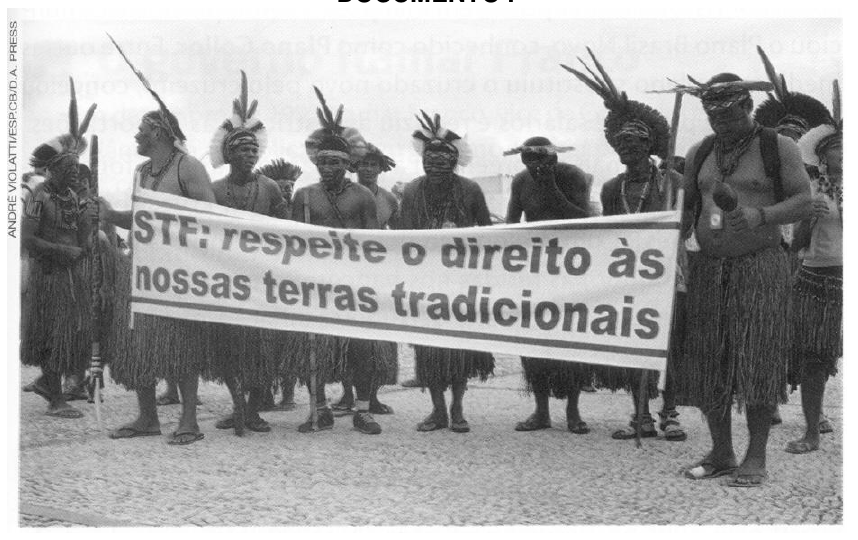
\includegraphics[width=0.95\linewidth]{static/simulados/coluni/figuras/2020/questao-36/figura-1.png}
\end{figure}
% COLUNI-AUTO-FIGURES-END

Indígenas realizam caminhada ao longo da Esplanada dos Ministérios em protesto contra a Proposta de Emenda Constitucional (PEC) 215/00, que transfere da União para o Congresso Nacional o poder de decidir sobre a demarcação das Terras Indígenas. Brasília (DF), 18 de março de 2015.

BRAICK, Patrícia Ramos. \textbf{Estudar História}: das origens do homem à era digital. 2. ed. São Paulo: Moderna, 2015, p. 241.

\textbf{DOCUMENTO II}

Na nossa terra temos muitas serras. Dentro das serras moram os xaporis, hekuras, os espíritos da natureza. As serras são lugares sagrados [...] onde os espíritos dos mortos retornam para viver. Os nossos velhos deixaram seus espíritos nesses lugares. Nós, yanomamis, queremos que as serras sejam respeitadas, não queremos que sejam destruídas.

ZENUN, Katsue H.; ADISSI, Valeria Maria A. Ser Índio hoje. São Paulo: Edições Loyola, 1998, p. 83. Apud BOULOS JÚNIOR, Alfredo. \textbf{História sociedade \& Cidadania}, 9º ano. 3. ed. São Paulo: FTD, 2015, p. 322.

Sobre a demarcação das Terras Indígenas no Brasil, é CORRETO afirmar que:
\begin{enumerate}
\item a Constituição de 1988 garante aos povos indígenas os direitos originários sobre as terras coletivas que
      eles ocupam tradicionalmente.
\item a maior parte das Terras Indígenas regularizadas localiza-se na região litorânea brasileira e pertence aos
      povos Guarani.
\item a demarcação das Terras Indígenas tem sido historicamente assinalada por um processo conflituoso e
      violento em função dos interesses indígenas na exploração de atividades ligadas ao agronegócio.
\item os significados simbólicos e espirituais relacionados às tradições indígenas são critérios secundários na
      demarcação das Terras Indígenas.
\end{enumerate}
